\chapter{Results}\label{cp:results}

\autoref{fig:deformed_truss} shows the deformed truss (colored) over the original truss (black). The supports and the applied point load are not shown. \autoref{tab:nodes} lists the displacement \gls{u} and force \gls{f} at each node. \autoref{tab:members} lists the internal stress \gls{sigma}, force \gls{f}, and \gls{v} for each member in the truss. The node and member numbers in \autoref{tab:nodes} and \autoref{tab:members} correspond to the nodes identified in \autoref{fig:deformed_truss}.

The raw text files output by Ansys which these tables were derived from can be found in \autoref{sec:ansys_output}.

\begin{figure}[htpb]
    \centering
    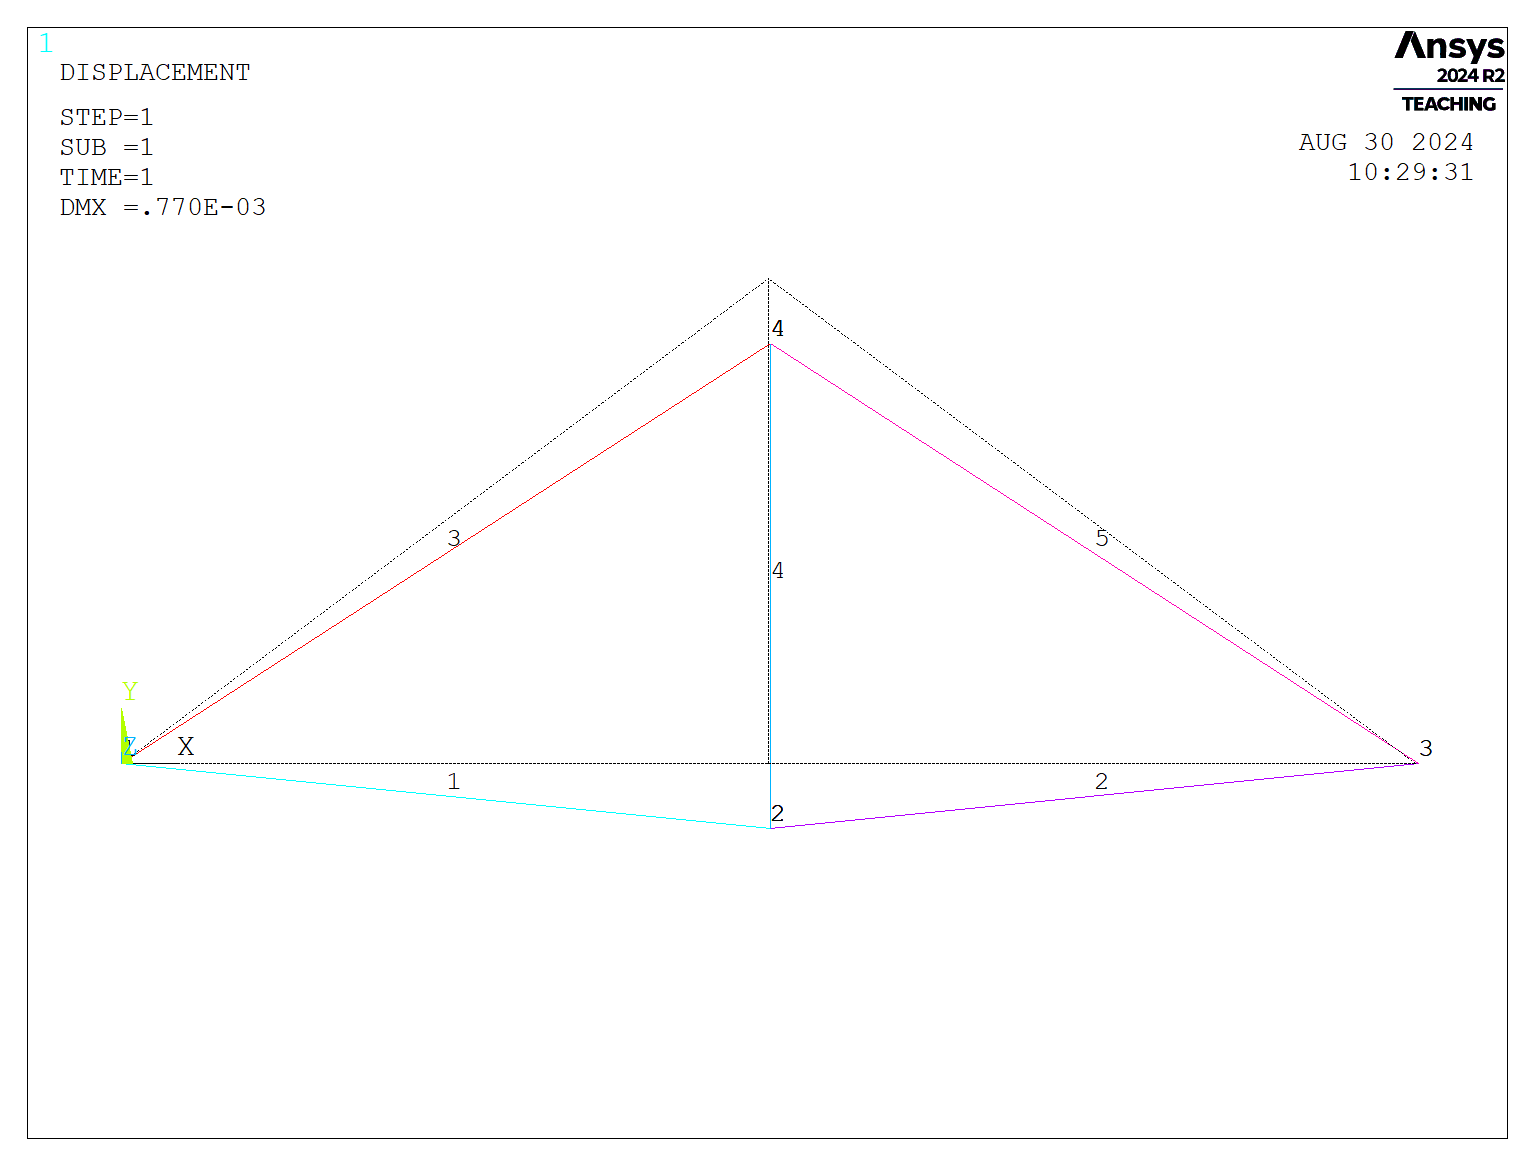
\includegraphics[width=\linewidth]{Figures/deformed_shape.png}
    \caption[The original and deformed truss]{The original truss (black outline) and deformed truss (colored outline).}
    \label{fig:deformed_truss}
\end{figure}

\begin{table}[htpb]
    \centering
    \caption[Nodal solutions]{The displacement \gls{u} and force \gls{f} at each node.}
    \begin{tabular}{cccccccc}
    \toprule
    Node & \gls{u_x} $\left[\unit{\micro\meter}\right]$ & \gls{u_y} $\left[\unit{\micro\meter}\right]$ & \gls{u_z} $\left[\unit{\micro\meter}\right]$ & $\left|\text{\gls{u}}\right|$ $\left[\unit{\micro\meter}\right]$ & \gls{f_x} $\left[\unit{\newton}\right]$ & \gls{f_y} $\left[\unit{\newton}\right]$ & \gls{f_z} $\left[\unit{\newton}\right]$ \\
    \midrule
    \num{1} & \num{0} & \num{0} & \num{0} & \num{0} & \num{0} & \num{750} & \num{0} \\
    \num{2} & \num{19.048} & \num{-769.44} & \num{0} & \num{769.68} & \num{0} & \num{0} & \num{0} \\
    \num{3} & \num{38.095} & \num{0} & \num{0} & \num{38.095} & \num{0} & \num{750} & \num{0} \\
    \num{4} & \num{19.048} & \num{-769.44} & \num{0} & \num{769.68} & \num{0} & \num{0} & \num{0} \\
    \bottomrule
\end{tabular}
    \label{tab:nodes}
\end{table}

\begin{table}[htpb]
    \centering
    \caption[Member solutions]{The internal stress \gls{sigma}, force \gls{f}, and volume \gls{v} for each individual member.}
    \begin{tabular}{cccc}
    \toprule
    Member & \gls{sigma} [\unit{\mega\pascal}] & \gls{f} [\unit{\kilo\newton}] & \gls{v} [\unit{\meter^3}] \\
    \midrule
    \numrange[range-phrase = --]{1}{2} & \num{4.00} & \num{1.00} & \num{0.250e-3} \\
    \bottomrule
\end{tabular}
    \label{tab:members}
    \vspace*{5in}
\end{table}